\section{System Overview}
As stated in the requirements, the system should handle streaming video from a camera, perform convolution and be able to provide the result as an output stream.
The convolution is to be done on the FPGA using a custom processor implementation named \textit{Daisy}, described in section \ref{sec:processor}.
To make the FPGA as simple as possible, the camera is connected to and controlled by the MCU, and the video is passed to the convolution processor in a suitable format over an EBI bus.

Furthermore, as HDMI output is not available on the MCU and the bus between the MCU and FPGA is already assumed to be a bottleneck, the HDMI output is placed on the FPGA.

Figure \ref{fig:systemArchitecture} displays the overall system architecture.

\begin{figure}
    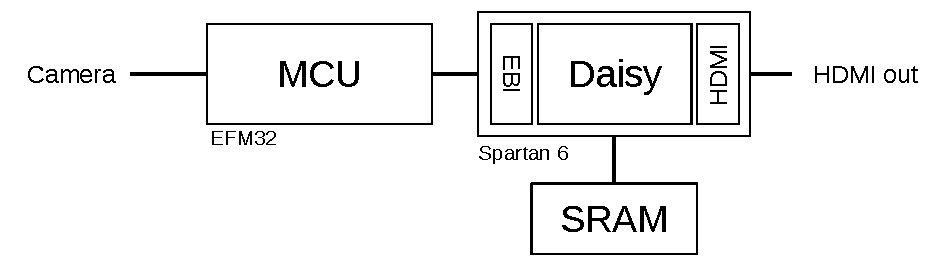
\includegraphics{img/SystemArchitecture.pdf}
    \caption{System Architecture}
    \label{fig:systemArchitecture}
\end{figure}



\subsection{Data Flow}
Notice how data flows from left to right in figure \ref{fig:systemArchitecture}.
The data we are going to process is first created by the camera and sent to the MCU.
The MCU may have to do some conversion should the camera provide the image in a format unsuitable for the processor, but will mainly be forwarding the data directly to the FPGA.
However, interfacing with the camera is assumed to be simpler to do from the MCU than from the FPGA as libraries most likely already exists.

On the FPGA, the data is received by an EBI controller which takes care of the protocol used on the bus and forwards data to the processor.
When data arrives at the processor, the convolution starts and the output is written to SRAM.

The SRAM is temporary storage to avoid synchronization issues between the FPGA and the HDMI controller.
Synchronization at this point would require the rest of the system to always be able to provide data at the exact rate provided by HDMI and was considered to be too risky.


\subsection{Backup Solutions} \label{subsec:RiskAssessment}
During the project, a risk assessment was done to find and reduce the risk of failure.
This lead to some backup solutions being implemented in the design.

One such solution was to exaggerate the number of address lines from the MCU to the FPGA to support addressing the memory connected to the FPGA directly (through the FPGA).
This will be useful should the communication directly from the MCU to the processor prove hard to establish.
This is a critical point because the data needs to cross clock domains correctly.

One of the measures taken was to add an extra HDMI port connected to the FPGA in case we failed to transfer video from the MCU to the FPGA or the throughput proved to be insufficient.
This allows us to connect the camera directly to the FPGA and circumvent both the EBI bus and the MCU, as shown in figure \ref{fig:SystemArchitectureAlternative}

Also shown in the figure is an extra SRAM chip.
The extra chip doubles the available throughput between the memory and the FPGA and reduces the chance of conflicts between the processor and the HDMI controller which will access the memory at the same time. Using double buffering, we can ensure they never access the same memory at the same time.

\begin{figure}
    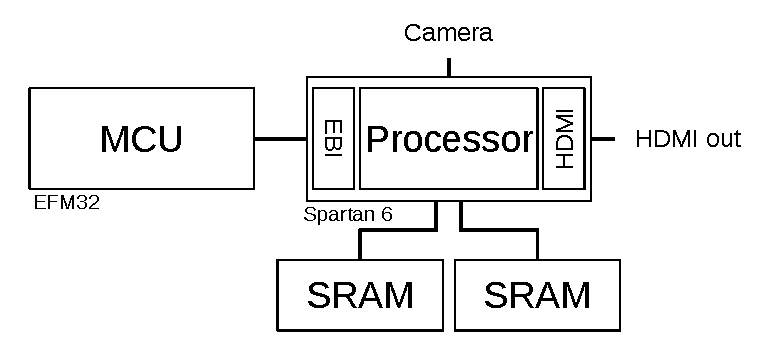
\includegraphics{img/SystemArchitectureAlternative.pdf}
    \caption{Alternative System Architecture}
    \label{fig:SystemArchitectureAlternative}
\end{figure}
